\chapter{Merkmalsextraktion}

\section{Verwendete Software}

Um die verschiedenen Verfahren zur Merkmalsextraktion zu vergleichen wurde ein Programm in C++ erstellt.
Also Entwicklungsumgebung wurde die freie und quellenoffene Software Eclipse verwendet.
Die genutzten Implementierungen der Bildverarbeitungsalgorithmen stammen aus der Bibliothek OpenCV. Hierbei handelt es sich um eine unter der BSD Lizenz veröffentlichten Software die sehr viele Methoden zur Bildverarbeitung und Maschinellem sehen enthält.

\section{Hardware}

Das Programm wurde auf einem Laptop mit folgender Hardware erstellt und getestet:
\begin{itemize}
\item Intel Core i7-4720HQ mit bis zu 3.6 GHz
\item 8 GB DDR3L-SDRAM mit 1600 MHz
\item Nvidia Geforce GTX 960M
\end{itemize}

Als Kamera wurde eine Logitech HD Pro C920 Webcam verwendet, da diese sich durch ein sehr gutes Preis-Leistungs Verhältnis auszeichnet.

\section{Erstellte Software}
Zum testen und vergleichen der drei behandelten Merkmalsverfahren wurde ein Programm erstellt, das mit Hilfe dieser durch Bilder vorgegebene Objekte in dem Videostream einer Webcam erkennt.
Der verwendete Algorithmus lässt sich durch das setzen einer Variable bestimmen. Dies ist zwar nicht so benutzerfreundlich wie die Übergabe eines Arguments beim Aufruf des Programms, da bei jeder Änderung neu kompiliert werden muss, aber für Testzwecke ist es ausreichend.
Nachdem die Header-Dateien der benötigten Bibliotheken eingebunden wurden, werden die Bilder der zu suchenden Objekte aus einem definierbaren Ordner geladen. Es können theoretisch beliebig viele Bilder in diesen Ordner eingefügt werden, es wurden aber maximal 6 gleichzeitig getestet.
Da der Autofocus der Webcam nicht sehr zuverlässig funktioniert, wurde eine Manuelle Focus Funktion in Form einer OpenCV Trackbar Implementiert. 
\begin{figure}[h]
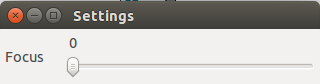
\includegraphics[width=0.6\textwidth]{trackbar.png}
\centering
\end{figure}
Um die Daten der Kamera verarbeiten zu können wird ein VideoCapture Objekt angelegt über das man die Mat-Container der einzelnen Frames beziehen kann.
Um die erkannten Objekte am besten Farblich darzustellen wird der Farbkreis in die Anzahl der zu erkennenden Objekte unterteilt. Das lässt sich am einfachsten im HSI Modell realisieren in dem jedes Objekt einen Hue wert:
\begin{equation}
H = i \cdot \dfrac{180}{\text{Anzahl der Objekte}} \\
\text{mit } 0 < i < \text{Anzahl der Objekte}
\end{equation}
Die so erhaltenen Farben werden anschließend in das RBG-Format umgerechnet und in einen Vektor für die spätere Verwendung gespeichert.
Da die Algorithmen auf Graustufenbildern arbeiten werden die Bilder der zu erkennenden Objekte konvertiert und in ein separates Array gespeichert.
Anschließend werden nach dem gewünschten Verfahren die Keypoints aus den Bildern extrahiert und die Deskriptoren berechnet.
Dies wird anhand der Methoden \emph{detect} und \emph{compute} der Klassen \emph{xfeatures2d::SIFT}, \emph{xfeatures2d::SURF} und \emph{ORB} bewerkstelligt. 
Falls bei diesem Schritt ein Fehler auftritt muss das betroffene Objekt in Form des zugehörigen Bildes, der Keypoints und der Deskriptoren aus den jeweiligen Vektoren gelöscht werden.
Dies ist insbesondere wichtig da die zu einem Objekt gehörenden Daten nur durch die Stelle in den Vektoren zusammenhängen.
Nachdem die Merkmale aus den Objektbildern extrahiert wurden, springt das Programm in eine nur durch die Beendung des Programms unterbrechbare Endlosschleife in der die aktuellen Frames der Webcam bearbeitet werden.
